\chapter{Wprowadzenie}
\thispagestyle{chapterBeginStyle}
\label{rozdzial1}
\section{Planowanie}

    Codziennie ludzie używają słowa "plan" w różnych kontekstach: firma planuje rozkład palet na magazynie, trener planuje strategię na
    najbliższy mecz, student planuje jak rozwiązać zadanie na kolokwium, czy chociażby człowiek codziennie planuje listę zakupów. \\
    Mimo różnych kontekstów istnieją wyodrębnione wspólne cechy każdego z planów:
    \begin{definition}
    \label{StanyPoczatkowe}
        \textbf{Warunki początkowe} - stan świata przed zastosowaniem akcji. W dalszej części pracy również określane jako 
        \textbf{stany początkowe}.
    \end{definition}
    \begin{itemize}
        \item Każdy plan musi mieć jasno zadeklarowane warunki początkowe.
        Dzięki dokładnej wiedzy o świecie możliwym jest poprawne określenie akcji, przy pomocy których wprowadzane są modyfikacje
        obecnego stanu aż do otrzymania zadowalających rezultatów. Dla przykładu, firma musi wiedzieć ile oraz jakie palety 
        przybędą na magazyn zanim rozpocznie planowanie rozkładu dostawy na magazynie.
    \end{itemize}
    \begin{definition}
    \label{Akcje}
        \textbf{Akcja} - działanie zmieniające przedstawiony świat w ściśle określony sposób. W dalszej części pracy również określana jako
        \textbf{operator}.
    \end{definition}
    \begin{itemize}
        \item Akcje pozwalają na modyfikację przedstawionego świata. Każda z akcji składa się z podmiotu, na który działa oraz czynności,
        która jest względem wskazanego podmiotu wykonywana. Przykładem dobrze określonej akcji może być przeniesienie klocka z 
        jednego stolika na drugi- składa się ona z podmiotu w postaci klocka, oraz czynności w postaci przenoszenia, które możemy traktować
        jako ruch. Czynności mogą różnić się od siebie w kwestii skomplikowania, najważniejszym jest, aby były określone poprawnie i aby były wykonalne w zdefiniowanym świecie.
    \end{itemize}
    \begin{definition}
    \label{Cel}
        \textbf{Cel} - Oczekiwany stan świata.
    \end{definition}
    \begin{itemize}
        \item Kwintesencją każdego planu jest cel, który należy uzyskać. Zwyczajowo plany składają się z celów możliwych do
        osiągnięcia ze stanu początkowego przy pomocy zdefiniowany operacji, jednakże trzeba wziąc pod uwagę sytuację, w której 
        niemożliwym jest uzyskanie wskazanego celu, szczególnie próbująć automatyzować pojęcie planowania.
    \end{itemize} 
    Przy pomocy powyższych definicji możliwym jest sformalizowanie pojęcia stojącego za słowem \textbf{plan}. 
    \begin{definition}
    \label{Plan}
    \textbf{Plan}- lista akcji, której zastosowanie do stanu początkowego powoduje jego zmianę do stanu określonego w ramach cel. 
    \end{definition}
    
    \begin{figure}[H]
        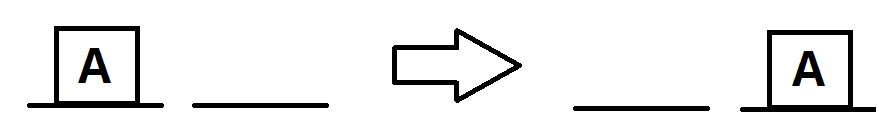
\includegraphics[scale=0.5]{Przyklad1}
        \centering
        \caption{Przeniesienie klocka z jednej półki na drugą jako przykład sytuacji
        dla której istnieje możliwość utworzenia planu. Po lewej stronie od strzałki znajduje się stan
        początkowy, natomiast po prawej- oczekiwany cel. Naturalną akcją w przedstawionym świecie jest akcja \textit{przenieś}, która
        zadany klocek przenosi z jednej półki na drugą.}
        \label{Przyklad1}
    \end{figure}
    Łatwo zauważyć na podstawie przykładu \ref{Przyklad1}, iż można utworzyć wiele planów, które dla zadanego stanu początkowego 
    osiągają wskazany cel. Dla powyżej sytuacji naturalnym planem jest przeniesienie klocka A z platformy po lewej na platformę po prawej, 
    lecz nie jest to jedyna możliwość. Również satysfakcjonującym planem zgodnie z wprowadzoną wyżej definicją byłaby następująca sekwencja
    akcji:
    \begin{enumerate}
        \item Przenieś klocek A z lewej platformy na prawą
        \item Przenieś klocek A z prawej platformy na lewą
        \item Przenieś klocek A z lewej platformy na prawą
    \end{enumerate}
    Generowanie rekruencyjne nieskończonych planów poprzez bezużyteczne przestawienia "w miejscu", mimo tego, iż zawiera się w definicji \ref{Plan},
    nie jest oczekiwanym efektem. Proces planowania odbywa się po to, by wykonać transformację świata przy jak najmniejszym
    nakładzie sił w jak najkrótszym czasie. Z tego względu wprowadzono pojęcie \textbf{planu optymalnego}.
    \begin{definition}
        \label{PlanOptymalny}
        \textbf{Plan optymalny}- Plan o minimalnej liczbie kroków satysfakcjonujący wskazany cel. 
    \end{definition}
     
    W dalszej części pracy słowo \textbf{plan} najczęściej będzie utożsamiane z planem optymalnym. \\
    Wprowadzenie powyższej definicji wiąże się z powstaniem bardzo ważnego pytania: \textit{Jak utworzyć plan optymalny?}. Bazując na przykładach
    takich jak \ref{Przyklad1} złudną może być myśl, iż generowanie optymalnych planów jest rzeczą prostą. Niech kolejny przykład będzie tego
    dowodem.
    \begin{figure}[H]
        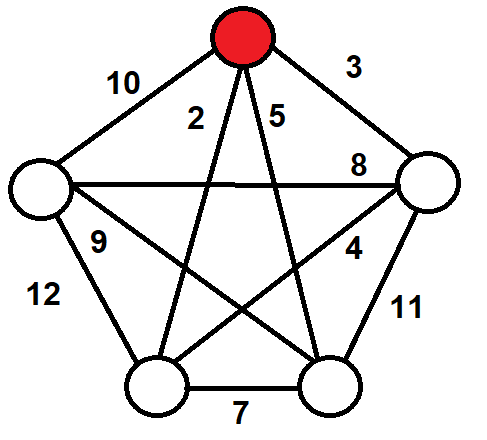
\includegraphics[scale=0.5]{Przyklad2}
        \centering
        \caption{Problem komiwojażera (Travelling Salesman Problem, TSP). Na rysunku pomocniczym liczby symbolizują wagi krawędzi. Węzeł oznaczony
        kolorem czerwonym odpowiada węzłowi startowemu, do którego należy wrócić. Długości krawędzi nie zachowują wskazanych przez wagi proporcji.}
        \label{TSP}
    \end{figure}
    Problem komiwojażera jest popularnym zagadnieniem optymalizacyjnym, którego istotą jest wskazanie ścieżki o najmniejszej sumie wag krawędzi, 
    która przechodzi dokładnie jeden raz przez każdy wierzchołek i wraca do wierzchołka startowego. Często problem wędrującego 
    komiwojażera przedstawiany jest przy pomocy kuriera oraz domów, które musi odwiedzić (za wierzchołek startowy uważa się magazyn,
    w którym kurier rozpoczyna swoją pracę). Mimo faktu, iż w przykładzie \ref{TSP} występuje jedynie 5 miejsc, 
    w których musi zatrzymać się kurier, utworzenie optymalnego planu dla przedstawionej sytuacji jest nielada wyzwaniem. Z tego powodu 
    ludzie postanowili skorzystać z potężnych mocy obliczeniowych komputerów przy generowaniu bardziej skomplikowanych planów.


\section{Planowanie przy użyciu komputerów}
    \subsection{STRIPS}
    W 1971 roku Panowie: Richard Fikes oraz Nils Nillson z Standford Research Institute (SRI International, 
    jeden z najsłynniejszych na świecie ośrodków badawczych) zdecydowali się na przedstawienie światu
    nowego podejścia w dziedzinie planowania o nazwie \textbf{STRIPS} (\textbf{ST}anford \textbf{R}esearch \textbf{I}nstitute
    \textbf{P}roblem \textbf{S}olver)\cite{STRIPS}.
    \textbf{STRIPS} rozwiązuje wskazany problem poprzez przeszukiwanie wszystkich stanów świata, aż do momentu
    gdy znajdzie taki, w którym wskazane cele są spełnione. Ważnym założeniem programu jest istnienie
    ciągu akcji, który gwarantuje otrzymanie celu. Zadanie to jest realizowane poprzez znalezienie
    sekwencji operatorów, która konwertuje wymodelowany stan początkowy, w model, w którym wszystkie 
    zdefiniowane cele są spełnione. Defnicje operatorów, stanu początkowego oraz celu są niemalże identyczne jak 
    \ref{StanyPoczatkowe}, \ref{Akcje} i \ref{Cel}, z tym, że definicja Akcji została w naturalny sposób rozwinięta o ciąg przyczynowo-skutkowy. Zauważono, iż w skład każdej akcji 
    poza samą czynnością wchodzą dwie składowe, nazywane środowiskowymi- warunki zajścia oraz efekty zajścia. 
    \begin{definition}
        \label{WarunekAkcji}
        \textbf{Warunkiem}- zajścia akcji jest istnienie odpowiedniej konfiguracji świata, dzięki której akcja może zostać wykonana.
    \end{definition}
    \begin{definition}
        \label{EfektAkcji}
        \textbf{Efektem}- zajścia akcji są zmiany, które zaszły w przedstawionym świecie ze względu na jej wykonanie.
    \end{definition}
    Mówiąc kolokwialnie, każda akcja ma swoją przyczynę oraz swój skutek. \textbf{Przyczyną} akcji w przykładzie \ref{Przyklad1} jest znajdowanie się klocka na lewej platformie. Gdyby
    klocek A znajdował się na prawej platformie, wykonanie akcji przesunięcia klocka z platformy lewej na prawą nie mogłoby zostać wykonane, natomiastem \textbf{efektem} akcji jest 
    przeniesienie klocka na prawą platformę. Łatwo zauważyć, iż brak innych obiektów na platformie prawej jest niezbędny, aby klocek mógł zostać tam przeniesiony.
    Kolejną naturalną obserwacją jest stwierdzenie, iż przeprowadzenie akcji dodaje nam nowe informacje o świecie w dwóch kontekstach:
    \begin{itemize}
        \item Dodającym- pojawienie się lub podtrzymanie danej składowej świata
        \item Usuwającym- pozbawienie świata danej składowej
    \end{itemize}
    Po wykonaniu czynności z przykładu \ref{Przyklad1} wyróżniamy trzy typy nowych informacji:
    \begin{itemize}
        \item Warunek dodający- Obecnośc klocka na lewej platformie, prawa platforma jest pusta
        \item Efekt dodający- Obecność klocka na prawej platformie
        \item Efekt usuwający - Platforma lewa jest pusta
    \end{itemize}
    W rozważanym podejściu każda z czynności zdefiniowana jest przy pomocy wyżej wskazanych trzech składowych.

        Takie zdefiniowane świata okazuje się wystarczające do rozwiązywania problemów pokroju rearanżacji obiektów czy 
    nawigowania w ściśle zdefiniowanej przestrzeni, czego najlepszym przykładem jest pierwszy robot- \textbf{Shakey}.
    Shakey był pierwszym robotem, który dzięki zainstalowanemu oprogramowaniu,
    posiadał umiejętność analizy własnego otoczenia. Dzięki zaimplementowanemu podejściu 
    STRIPS (oczywiście z odpowiednimi dostosowaniami do sytuacji) był w stanie rozwiązywać problemy z zakresu wyznaczania drogi,
    czy planowania rozmieszczenia obiektów w pokojach.
    Shakey, ze względu na swoją innowacyjność i przełomowość często jest nazywany archetypem
    dzisiejszych autonomicznych samochód czy militarnych dronów.

    Dzięki swojej roli w rozwoju planowania z użyciem komputerów, STRIPS został dodatkowo wyróżniony- od jego nazwy pochodzi języki opisu świata korzystający
    z trójki: stan początkowy, akcja oraz cel. Przez następne lata rozwiązania w obszarze planowania silnie bazowały na wprowadzonym w powyższej pracy opisie świata.

    \subsection{ADL i PDDL}
    TO-DO



    \subsection{Nowoczesne rozwiązania}
    TO-DO
    
    Pomiędzy powstaniem ulepszeń metodologii STRIPS w postaci ADL oraz PDDL powstały również inne podejścia, w tym
    silnie bazujący na grafach i ich możlwościach algorytm o wdzięcznej nazwie \textbf{GRAPHPLAN}






